\setlength\abovedisplayskip{2.5pt}

For relevant nuclear forensics predictions, both classification and regression
algorithms must be used.  For example, one may want to predict the reactor type
label given some measurement-based features of \gls{SNF} of an unknown source.
This would require a classification algorithm. Or perhaps the input fuel
composition is relevant to an investigation on weapons intent, so a regression
algorithm would be used. 

\subsubsection{Nearest Neighbor Methods}

Nearest neighbors classification and regression are unique algorithms in
that thay are instance-based; they do not actually generalize, but instead
track the observations in the training set.  The main metric for this algorithm
is distance (or dissimilarity) between the test sample and the closest training
sample(s) in the vicinity.  During prediction, the algorithm will calculate a
value based on the instance that is closest to the current test sample. Thus,
there is not any learning, but instead a direct comparison between an unknown
sample and the space that the training set populates. The predictions from
nearest neighbors can be quite accurate, but are highly unstable to
peturbations \cite{elements_stats}.

\begin{figure}[!htb]
  \centering
  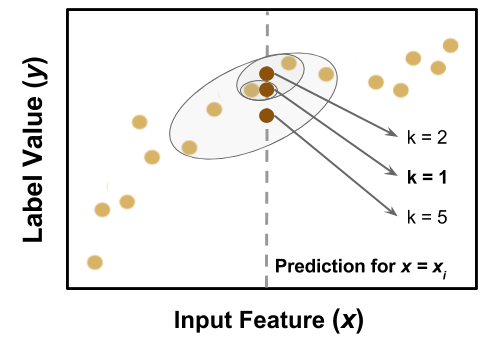
\includegraphics[width=0.8\linewidth]{./chapters/litrev/nn-fig.png}
  \caption{Schematic of \textit{k}-nearest neighbors regression, showing how 
           changing \textit{k} alters the predicted label value $y$.}
  \label{fig:nn}
\end{figure}

An extension of nearest neighbor is \textit{k}-nearest neighbor regression.
The closest \textit{k} neighbors are averaged for an estimate of the unknown
sample, as shown in Equation \ref{eq:knn}.  Figure \ref{fig:nn} provides a
pictoral explanation of how this is done for a prediction of a single feature.
For \textit{k}-neighbors, this algorithm predicts a value, $Y$, from the input
features, $\boldsymbol{X}$, in the neighborhood, $N_k (\boldsymbol{X})$
\cite{elements_stats}. 

\begin{equation}
  Y(\boldsymbol{X}) = \frac{1}{k} \sum_{x_i \in N_k(\boldsymbol{X})} y_i
  \label{eq:knn}
\end{equation}

There are two tuneable parameters in this algorithm: the distance metric and
the value of \textit{k}.  The population of the neighborhood, \textit{k},
affects the number of points being averaged together for a prediction.  The
metrics for distance can be the Manhattan distance, Euclidian distance, 
\todo[inline]{finish me}

\subsubsection{Decision Trees}



\subsubsection{Maximum Log-Likelihood Calculations}

The \gls{MLL} calulations approach applied here is based on a method developed
to do similar work \cite{mll_method, mll_validate, mll_sensitivity}.  That work
involved matching nuclear material samples based on some select measurements to
entries in a database of containing those measurements.\todo{keep vague or no?}
Each database entry also has a similar list of labels to the labels being
predicted in this work: reactor type, burnup, and time since irradiation.

Here, the same approach is taken. An "unknown" test sample is compared against
the training set using the likelihood calculation between that sample and the
training set entries.  The higher the likelihood, the higher the probability
that the database entry represents the sample. The likelihood is in Equation
\ref{eq:like}, whereas the log-likelihood is used more often in practice, shown
in Equation \ref{eq:loglike}.
\begin{equation}
  L(M|x_{test}) = \prod_i \frac{1}{\sigma_{i,sim} \sqrt{2\pi}} \exp{\frac{-(x_{i,test} - x_{i,sim})^2}{2 \sigma_{i,sim}^2}}
  \label{eq:like}
\end{equation}
\begin{equation}
  ln(L(M|x_{test})) = \sum_i ln(\frac{1}{\sigma_{i,sim} \sqrt{2\pi}}) - \frac{(x_{i,test} - x_{i,sim})^2}{2 \sigma_{i,sim}^2}
  \label{eq:loglike}
\end{equation}
The likelihood is a measure of the probability that a model $M$ produced the
measurements seen in the test sample, given by $L(M|x_{test})$.  In both
Equations \ref{eq:like} and \ref{eq:loglike}, $x$ refers to the set of
features, and $x_{i, test}$ and $x_{i,sim}$ are the individual features for the
test sample and the training set entries, respectively. The uncertainty of the
measurement associated with each feature is represented by $\sigma_{i,sim}$

\todo[inline]{Discuss how using a normal probability density function to match
the variables assume that the variables themselves are normal?}

Interestingly, the \gls{MLL} calculations method works like \textit{k}-nearest
neighbors, where there is no model but a prediction according to the closest
match database entry.  There is one detail that differs, however. Whereas
\textit{k}-nearest neighbors minimizes distance/dissimilarity, this approach
instead maximizes similarity via a likelihood function. 

